\documentclass[show notes]{beamer}

\usetheme{simple}

\usepackage{lmodern}
\usepackage[scale=2]{ccicons}


\title{Estimation problems in complex field studies with deep interactions}
\subtitle{time-to-event and local regression models for environmental effects on vital rates}
\author{Krzysztof Sakrejda}
\institute{Organismic and Evolutionary Biology \\ University of Massachusetts, Amherst}

\begin{document}

\maketitle


\begin{frame}{environmental effects}
  \framesubtitle{motivation}

	\begin{figure}
	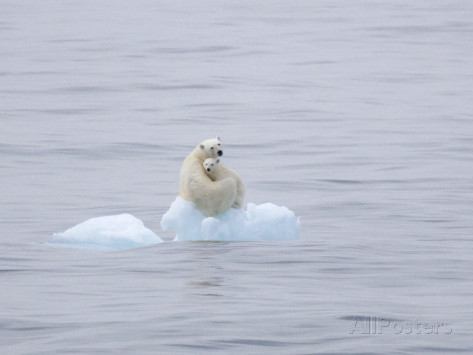
\includegraphics[width=.8\textwidth]{bears-on-ice.jpg}
  	\end{figure}
  
\end{frame}

\begin{frame}{forecasting}
  \framesubtitle{broad interest in forecasting biological systems}

	\begin{figure}
	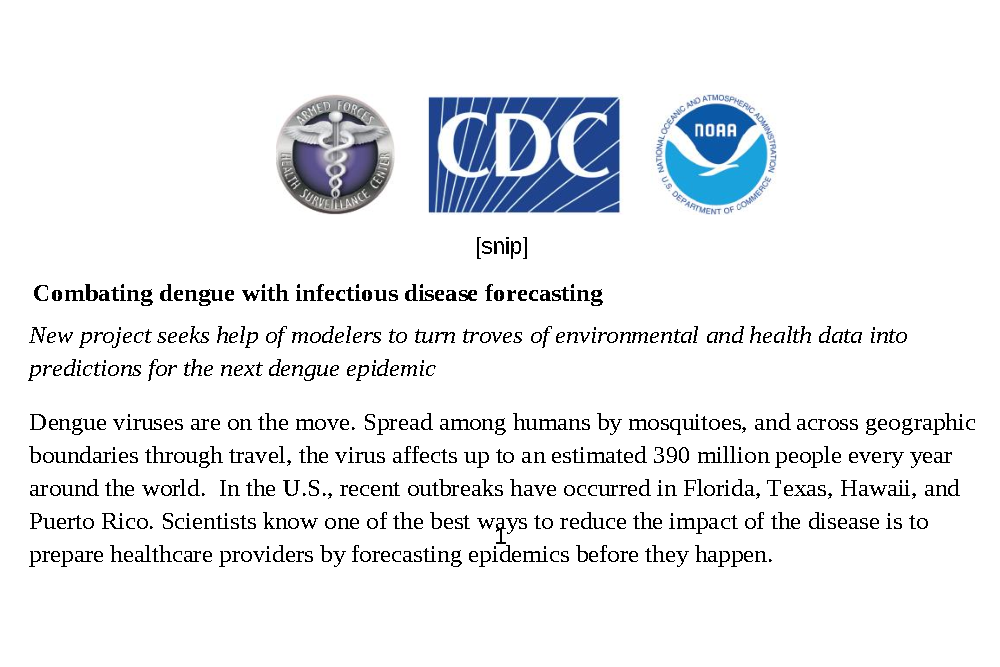
\includegraphics[width=\textwidth]{dengue-forecast-challenge.pdf}
  	\end{figure}
  
\end{frame}



\begin{frame}{forecasting}
  \framesubtitle{truism of forecasting that simple models work best}

	\begin{figure}
	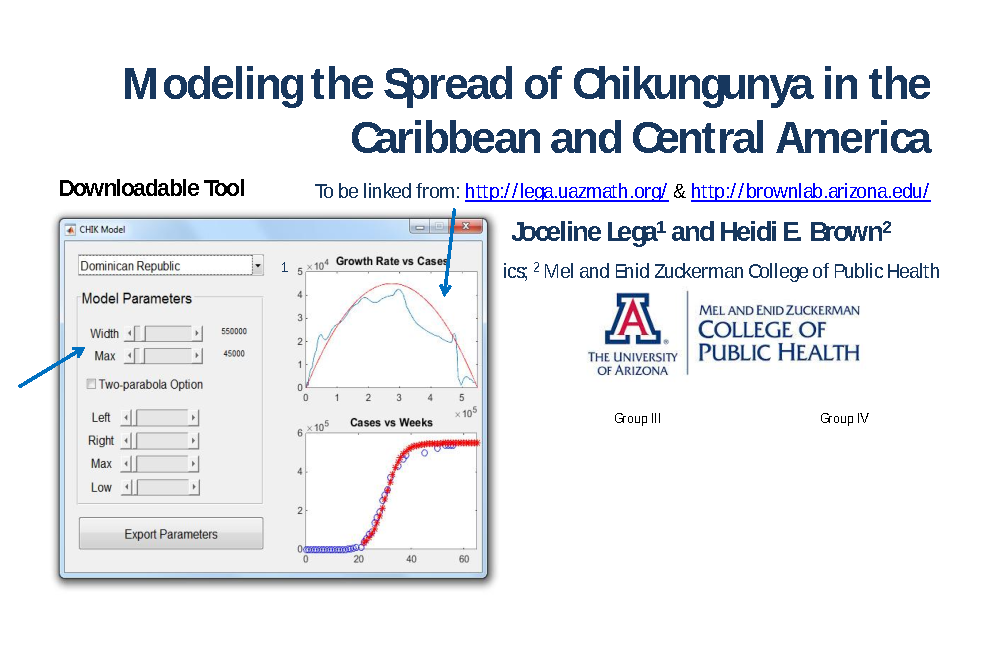
\includegraphics[width=\textwidth]{chikungunja-forecast-challenge.pdf}
  	\end{figure}
  
\end{frame}

\begin{frame}{how are ecologists doing?}
  \framesubtitle{we got a good start over 14 years ago.} 
  
  \begin{figure}
  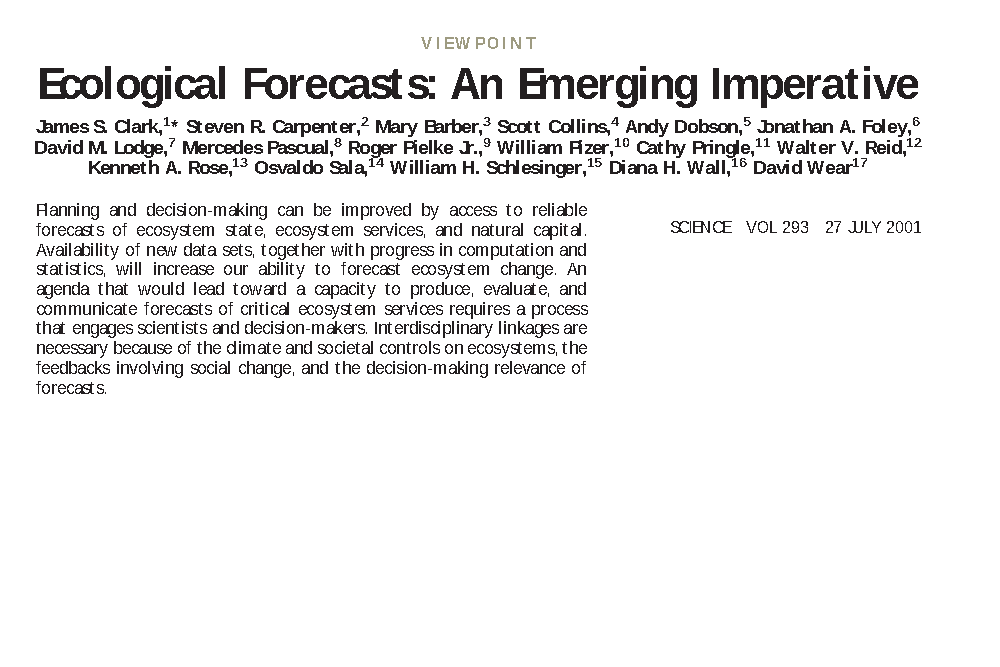
\includegraphics[width=\textwidth]{forecasts-are-good.pdf}
  \end{figure}
  
\end{frame}

\begin{frame}{how are ecologists doing?}
  \framesubtitle{simple may not do it for us} 
  
  \begin{figure}
  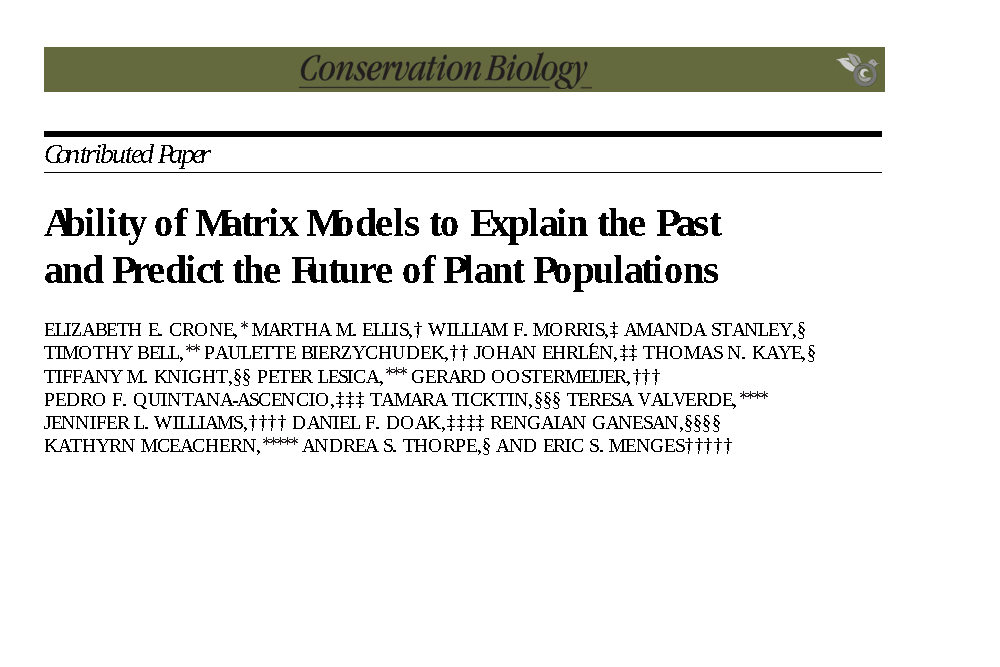
\includegraphics[width=\textwidth]{matrix-model-prediction.pdf}
  \end{figure}
  
\end{frame}



\begin{frame}{how are ecologists doing?}
  \framesubtitle{solid models based on solid data.} 
  
   \begin{itemize}
   \item 82 well studies plant populations
   \item 20 species over 3 continents
   \item parametrized stage-based matrix models
   \item evaluated in-sample accuracy
   \item generated five-year out-of-sample forecasts
   \end{itemize}
  
\end{frame}



\begin{frame}{how are ecologists doing?}
  \framesubtitle{disappointing performance} 
 
  \begin{figure}
  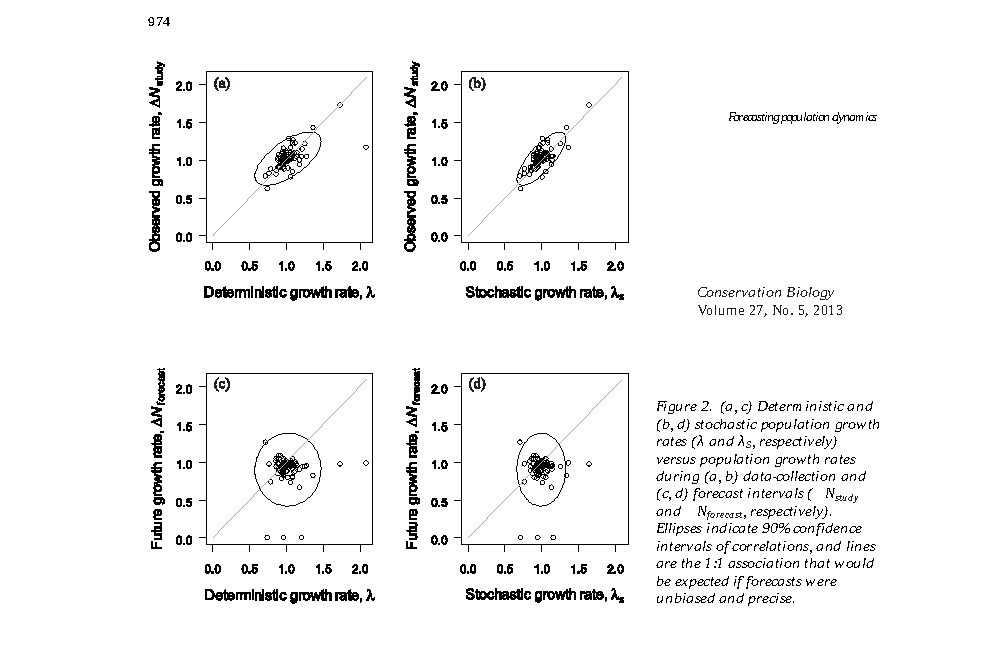
\includegraphics[clip, trim=50 0 0 0, width=\textwidth]{prediction-fail-figure.pdf}
  \end{figure}
  	
\end{frame}



\begin{frame}{how are ecologists doing?}
  \framesubtitle{maybe a little more complicated would help.} 
  
   \begin{itemize}
   \item nice in-sample prediction.
   \item dismal out-of-sample performance.
   \item ``only 40\% of observed population sizes fell within our forecasts' 95\% confidence limits.''
   \item ``Forecast error was significantly associated with environmental differences between the data collection and forecast periods.''
   \end{itemize}
\end{frame}




\begin{frame}{how are ecologists doing?}
  \framesubtitle{maybe a little more complicated would help.} 
   \begin{itemize}
   \item strict out-of-sample tests are both brutal and critical.
   \item strict out-of-sample tests are \emph{rare}.
   \end{itemize}
\end{frame}



\begin{frame}{species distribution models to the rescue.}
  \framesubtitle{simple models and ``cheap'' data.} 
  
  \begin{columns}
  \begin{column}{.4\textwidth}
   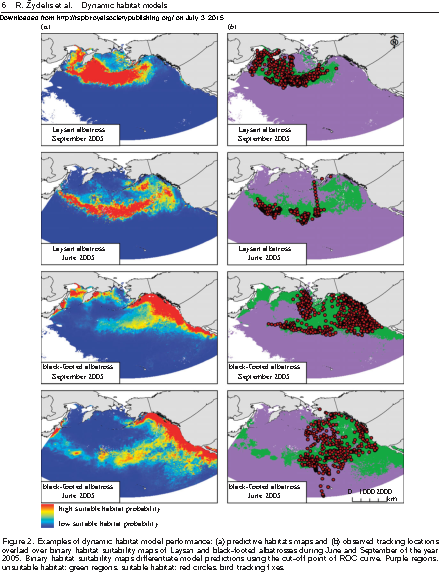
\includegraphics[width=\textwidth]{habitat-suitability.pdf}
  \end{column}
  \begin{column}{.6\textwidth}
  	\begin{itemize}
    \item point pattern of sp. observations
    \item spatial layers of environmental covariates
    \item GLM(M)'s, GAM, neural nets, etc...
    \item used for out-of-sample predictions
    \item \emph{evaluated} with out-of-sample prediction
    \end{itemize}
  \end{column}
  \end{columns}
\end{frame}


\begin{frame}{species distribution models to the rescue.}
  \framesubtitle{how do we assess what is good for prediction.} 
  
  \begin{columns}
  \begin{column}{.4\textwidth}
   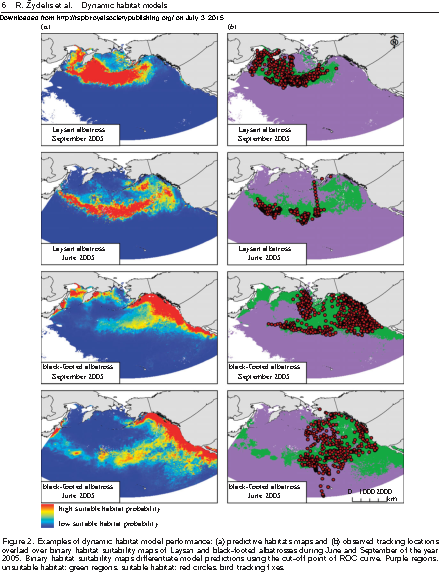
\includegraphics[width=\textwidth]{habitat-suitability.pdf}
  \end{column}
  \begin{column}{.6\textwidth}
	Randin et al. (2006) and Sundblad et al. (2009): 
  	\begin{itemize}
    \item data on 54 plant species with topographic and climate variables
	\item assessed bi-directional transferability of SDM's
    \item transferability varied widely by species
    \item models for only 50-70\% of species were transferable
    \item transferability can be directional
    \end{itemize}
  \end{column}
  \end{columns}
\end{frame}


\begin{frame}{species distribution models to the rescue.}
  \framesubtitle{what's eating your predictive power.} 
   
   Randin/Sundblad/out-of-sample quotes
   \begin{itemize}
   \item chains of correlations
   \item structured over-fitting
   \item in-sample vs. out-of-sample species and environmental mismatch
   \note[item]<1>{Mechanism is missing.}
   \note[item]<1>{Mechanistic parameters are missing.}
   \end{itemize}

\end{frame}


\begin{frame}{individual based models to the rescue.}
  \framesubtitle{I told you so.} 

\begin{quote}
"We have argued that the aggregation of individuals 
into large-scale population variables often glosses over mechanisms and 
variability at the level of individual interactions that are crucial 
to the larger-scale behavior of populations, communities, and ecosystems"
\end{quote}
Houston, DeAngelis, Post (1988)
  
\end{frame}

\begin{frame}{individual based models to the rescue.}
  \framesubtitle{everything should be fine then.} 

\begin{quote}
"These are the kinds of data that are commonly collected 
by autecologists, population ecologists, ecophysiologists, and some 
ecosystem ecologists. Thus it is feasible to obtain the parameters needed 
for [IBM's], in contrast with state-variable models for 
which processes must be measured at large scales, extrapolated from 
small-scale data, or derived by model fitting to obtain the needed input parameters."
\end{quote}
Houston, DeAngelis, Post (1988)

\end{frame}

\begin{frame}{What is an IBM.}
	\framesubtitle{paradise for lovers of box diagrams.}
    
    \begin{enumerate}
    \item define individual use of the environment, interactions with others, resource needs
    \item define the composition of a starting population
    \item use stochastic simulation to predict the future fate of individuals and their offspring
    \item aggregate the individual fates to predict ecosystem-level outcomes
    \end{enumerate}
    

\end{frame}

\begin{frame}{Atlantic salmon}
	\framesubtitle{do we know enough for an IBM?}
    
    Known knowns:
    \begin{enumerate}
    \item triggers for life events.
    \item competitive behaviors.
    \item feeding behaviors.
    \item social structure.
    \item physiological limits to growth and survival.
    \item physiological 
    \end{enumerate}


\end{frame}

\begin{frame}{MORE SALMON STUFF JUST T/D EFFECTS ON SURVIVAL}
\end{frame}



\begin{frame}{environmental conditions}
  \framesubtitle{stream discharge and water temperature}	
  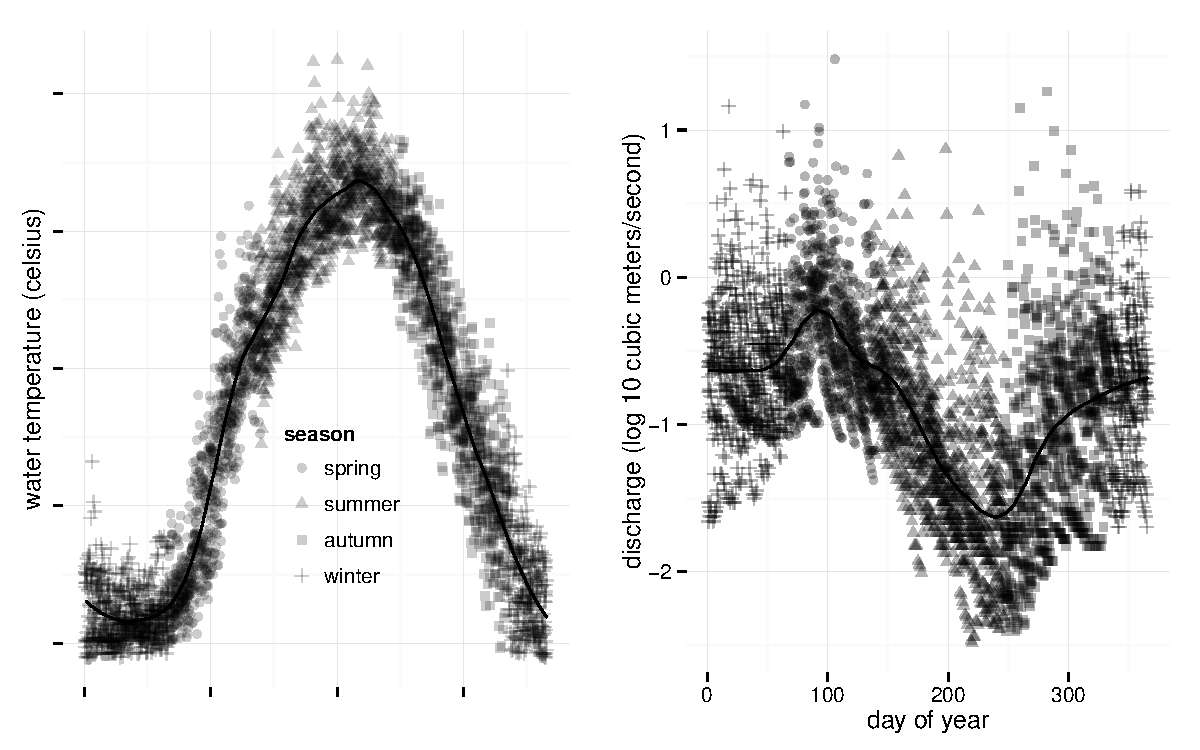
\includegraphics[clip, trim=0 0 0 0, height=.8\textheight]{pl-environment-wide.pdf}
    
\end{frame}

\begin{frame}{global models}

\begin{table}
\begin{center}
$
\begin{array}{lllll}
	Model \# & Survival                                                                          & Recapture                              & Smolting & Emigration \\
	0        & \phi_S                                                                            & p_S                                    & \alpha_S & \rho_S     \\
	1        & \phi_S                                                                            & p(d,4)                                 & \alpha_A & \rho_S     \\
	2        & \phi_{A\times S}                                                                  & p(d,4)                                 & \alpha_A & \rho_S     \\
	3        & \phi_{A\times S}                                                                  & p(d,4) + p_{OCC}                       & \alpha_A & \rho_S     \\
	4        & \phi_{A\times S} + \phi_{A+A:S}(T) + \phi_{A+A:S}(F) + \phi_{S}(T\times F)        & p(d,4)                                 & \alpha_A & \rho_S     \\
	5        & \phi_{A\times S} + \phi_{A+A:S}(T) + \phi_{A+A:S}(F) + \phi_{S}(T\times F)        & p(d,4) + p_{OCC}                       & \alpha_A & \rho_S     \\
	6        & \phi_{A\times S} + \phi_{A+A:S}(T)^2 + \phi_{A+A:S}(F)^2 + \phi_{S}(T \times F)^2 & p(d,4) +  p_{OCC}                      & \alpha_A & \rho_S     \\
	7        & \phi_S                                                                            & p(d,4) + p(dT) + p(d\log(F))           & \alpha_A & \rho_S     \\
	8        & \phi_{A\times S}                                                                  & p(d,4) + p(dT) + p(d\log(F))           & \alpha_A & \rho_S     \\
	9        & \phi_{A\times S}                                                                  & p(d,4) + p(dT) + p(d\log(F)) + p_{OCC} & \alpha_A & \rho_S     \\
	10       & \phi_{A\times S} + \phi_{A+A:S}(T) + \phi_{A+A:S}(F) + \phi_{S}(T\times F)        & p(d,4) + p(dT) + p(d\log(F))           & \alpha_A & \rho_S     \\
	11       & \phi_{A\times S} + \phi_{A+A:S}(T) + \phi_{A+A:S}(F) + \phi_{S}(T\times F)        & p(d,4) + p(dT) + p(d\log(F)) + p_{OCC} & \alpha_A & \rho_S     \\
	12       & \phi_{A\times S} + \phi_{A+A:S}(T)^2 + \phi_{A+A:S}(F)^2 + \phi_{S}(T \times F)^2 & p(d,4) + p(dT) + p(d\log(F)) + p_{OCC} & \alpha_A & \rho_S
\end{array}
$
\end{center}
\end{table}

    
\end{frame}




\begin{frame}{seasonal age-specific survival}
  \framesubtitle{modified cjs, global response model}

	\begin{figure}
	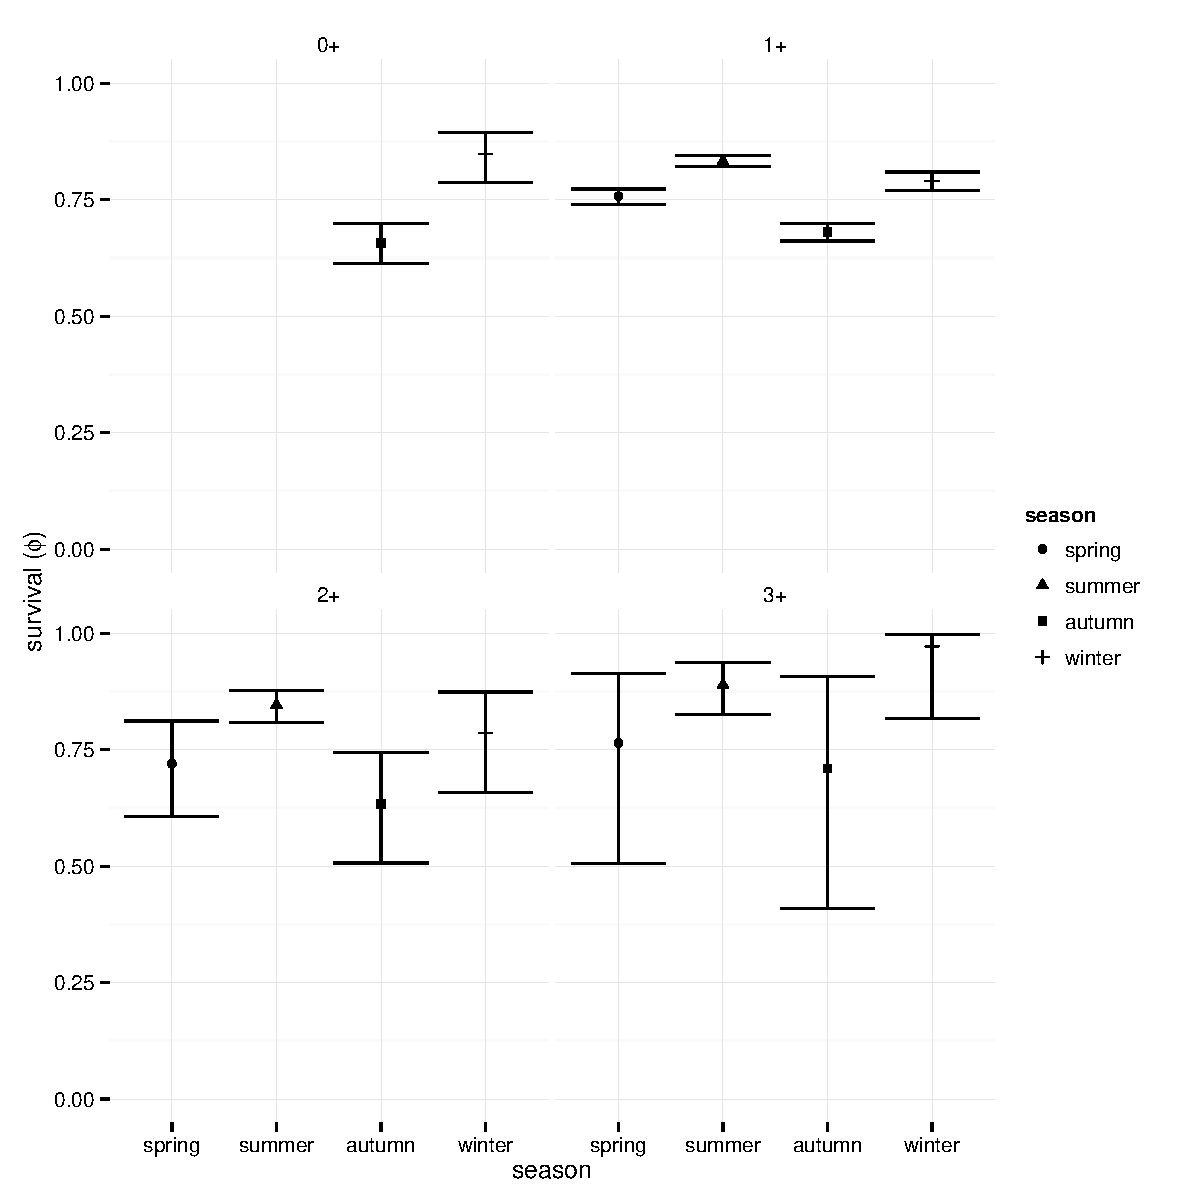
\includegraphics[clip, trim=0 0 0 10, height=.8\textheight]{pl-phi-age-x-season.pdf}
  	\end{figure}

\end{frame}


\begin{frame}{survival response surface}
  \framesubtitle{modified cjs, global response model}

	\begin{figure}
	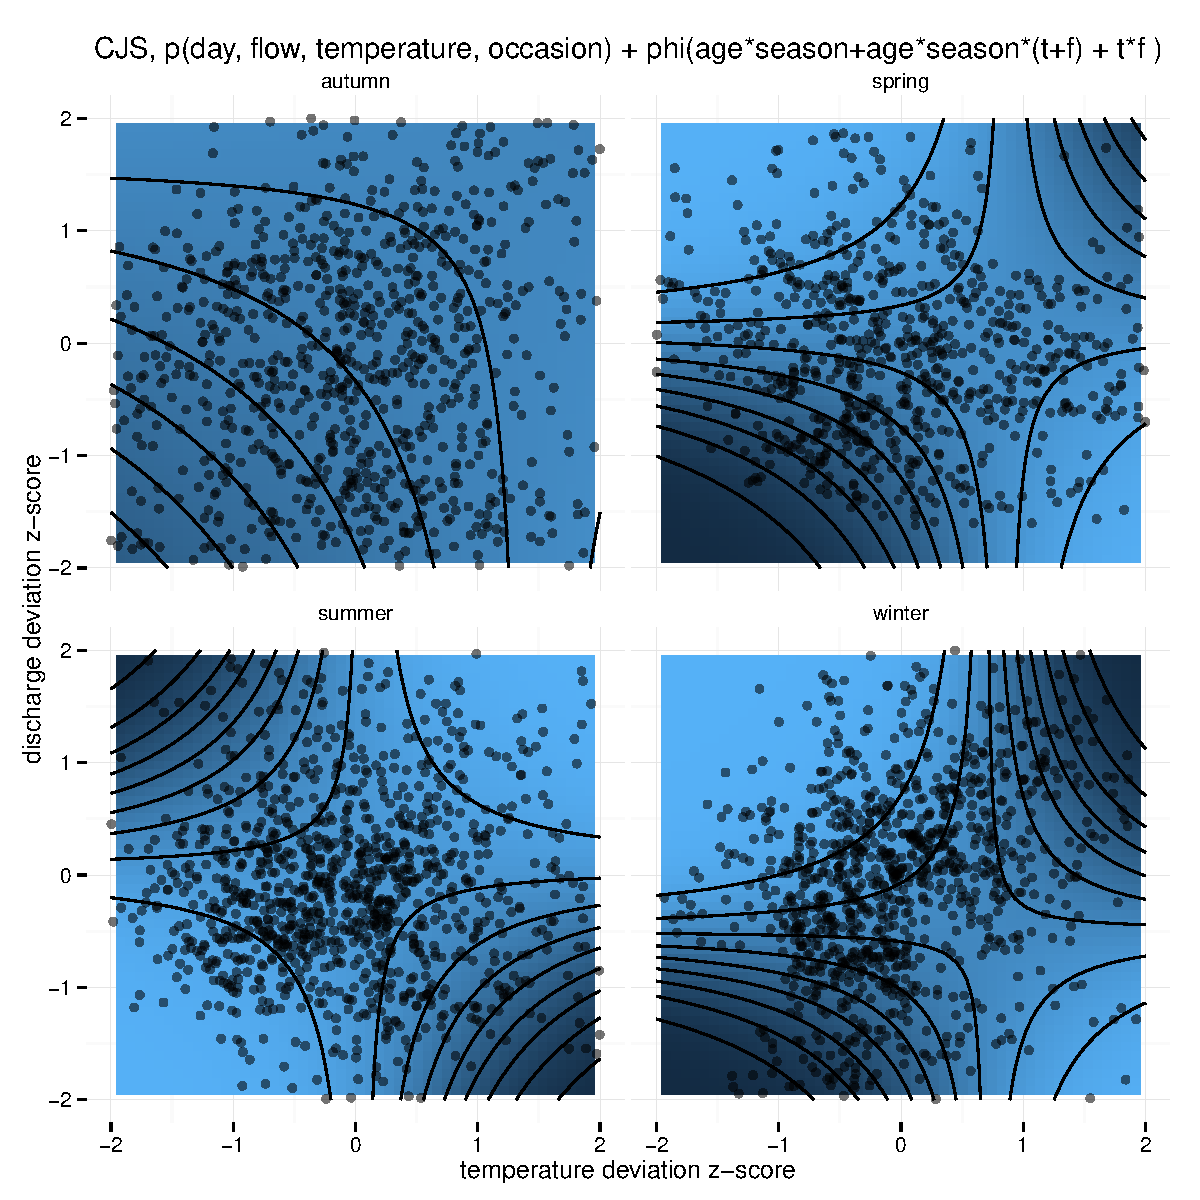
\includegraphics[clip, trim=0 0 0 35, height=.8\textheight]{pl-1-1-cjs-seasonal-logit-recapture_full_RE-phi_full_x-phi-heat-map.pdf}
  	\end{figure}

\end{frame}


\begin{frame}{timing of emigration}
  \framesubtitle{slow}	
  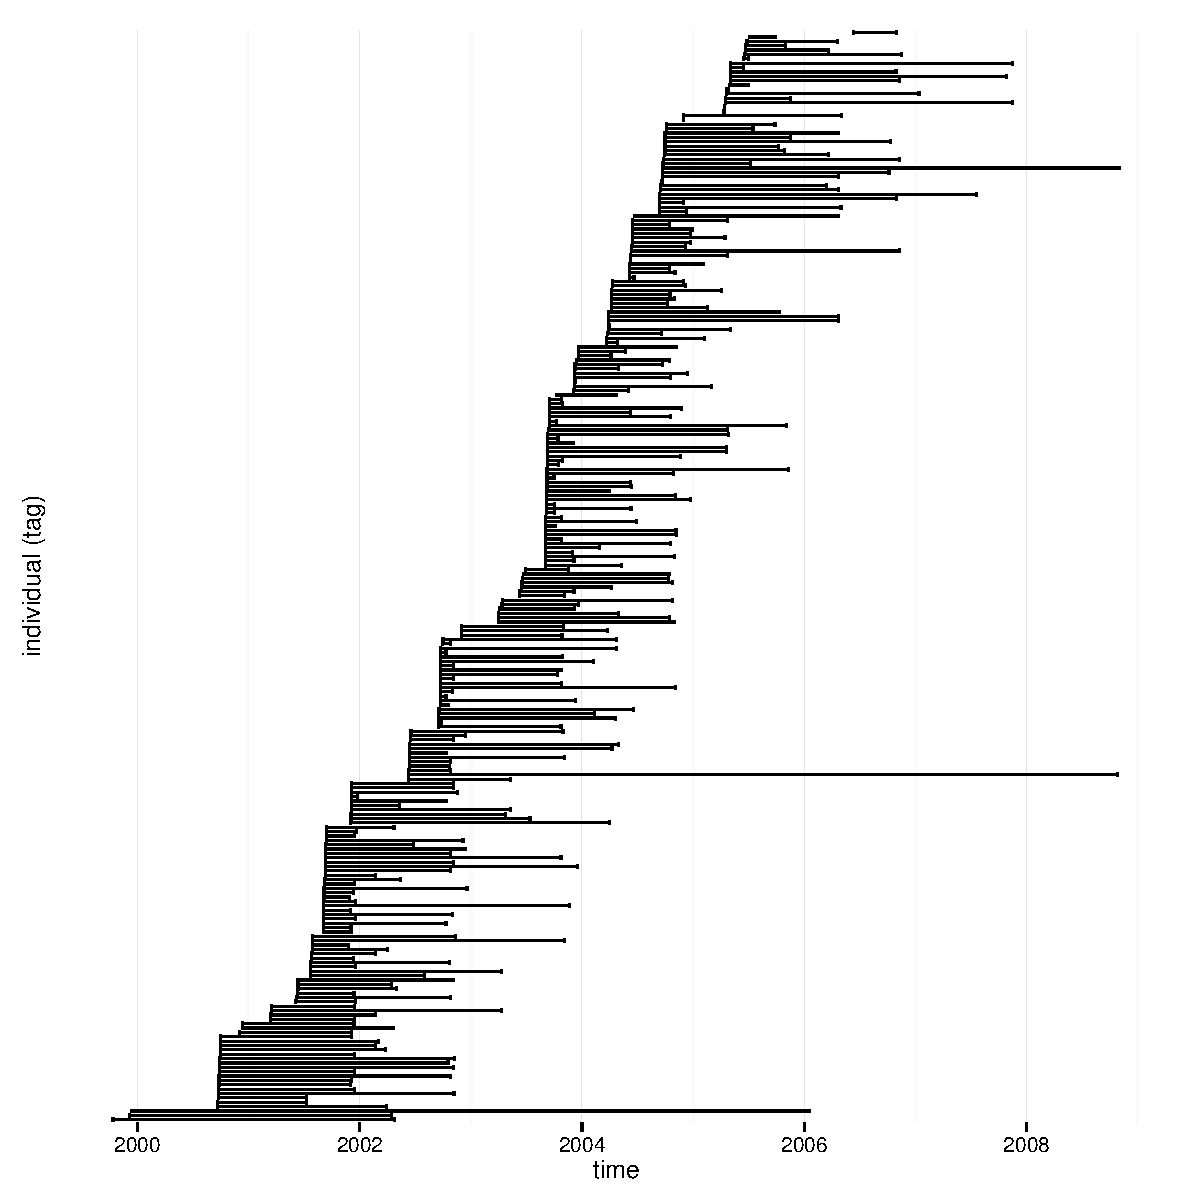
\includegraphics[clip, trim=0 0 0 0, height=.8\textheight]{emigrant-tracks.pdf}
    
\end{frame}

\begin{frame}{timing of emigration}
  \framesubtitle{slow}	
  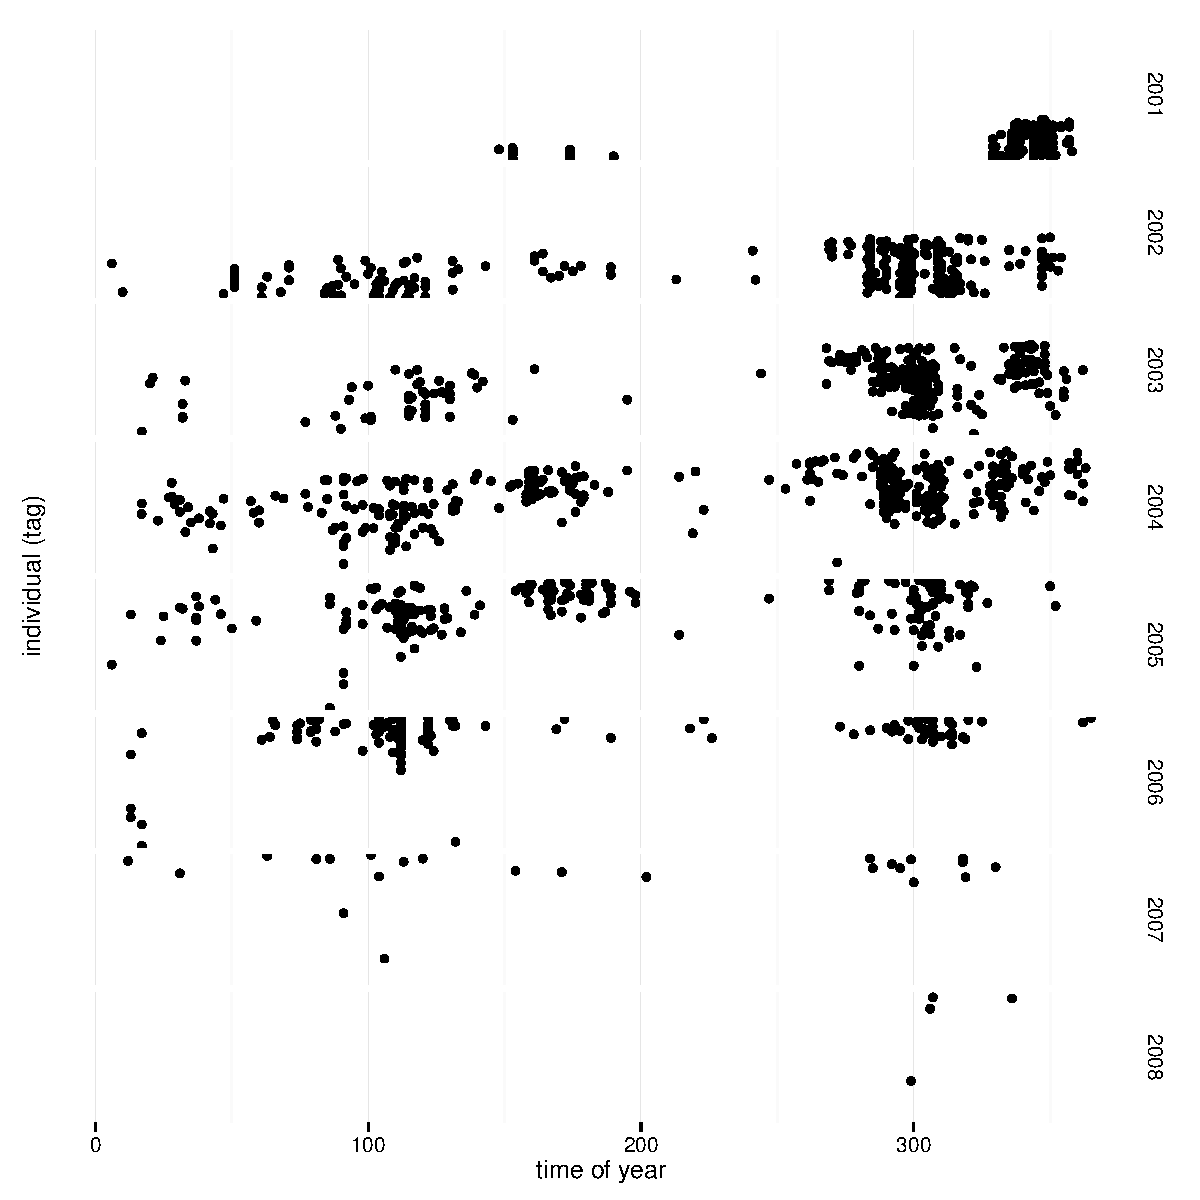
\includegraphics[clip, trim=0 0 0 0, height=.8\textheight]{emigrant-timing.pdf}
    
\end{frame}

\begin{frame}{timing of emigration}
  \framesubtitle{slow}	
  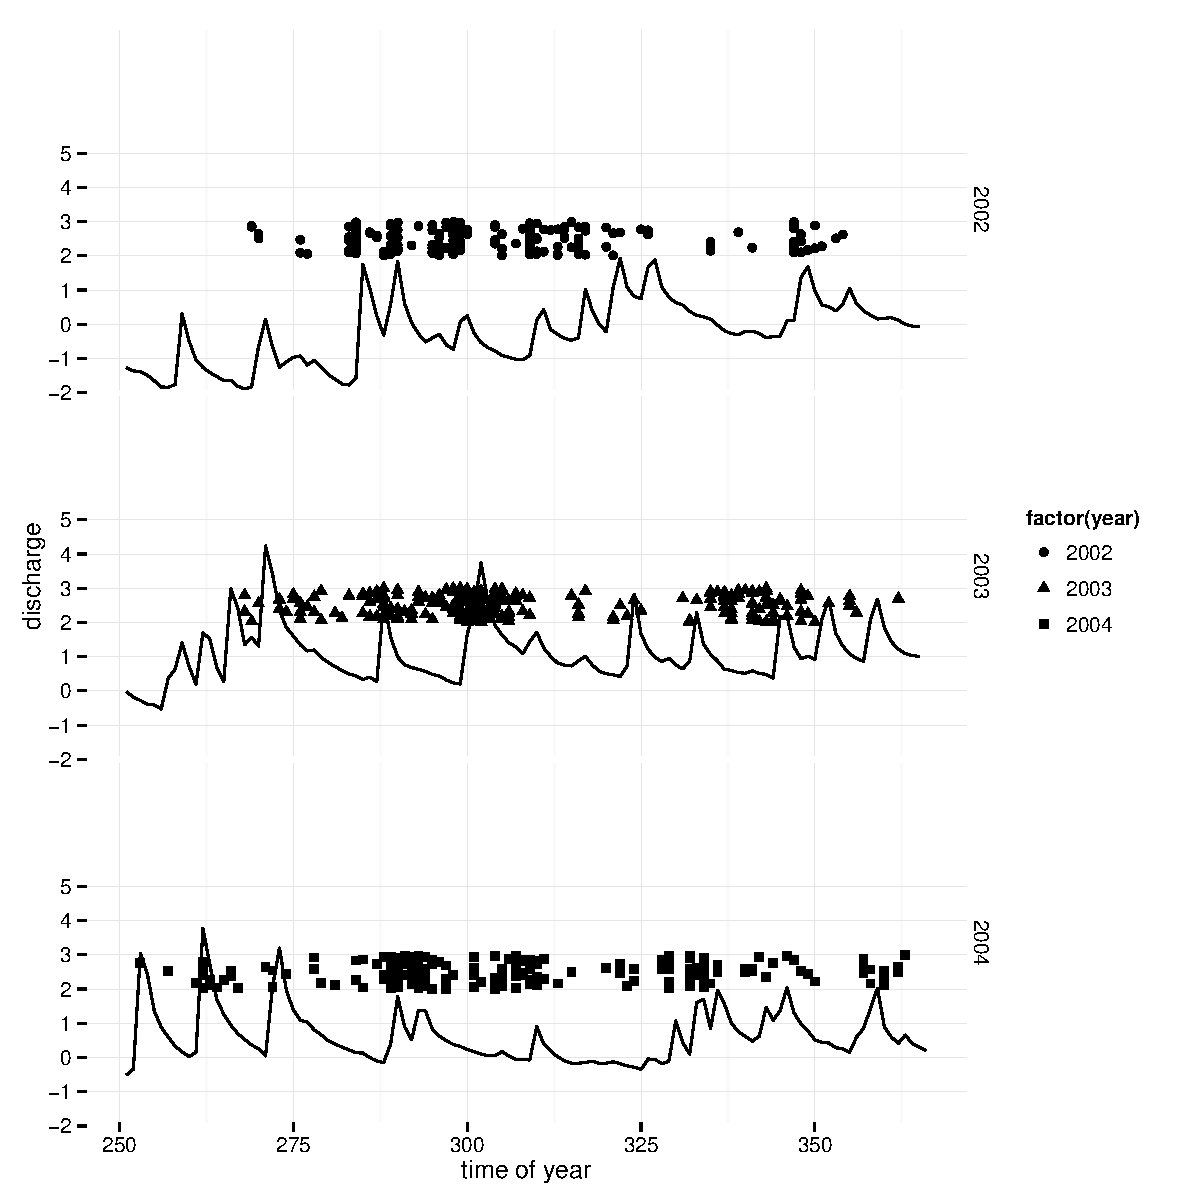
\includegraphics[clip, trim=0 0 0 0, height=.8\textheight]{emigrant-fast-events.pdf}
    
\end{frame}



\begin{frame}{(slow) temporal variation in emigration}
  \framesubtitle{samples of intensity function}

	\begin{figure}
	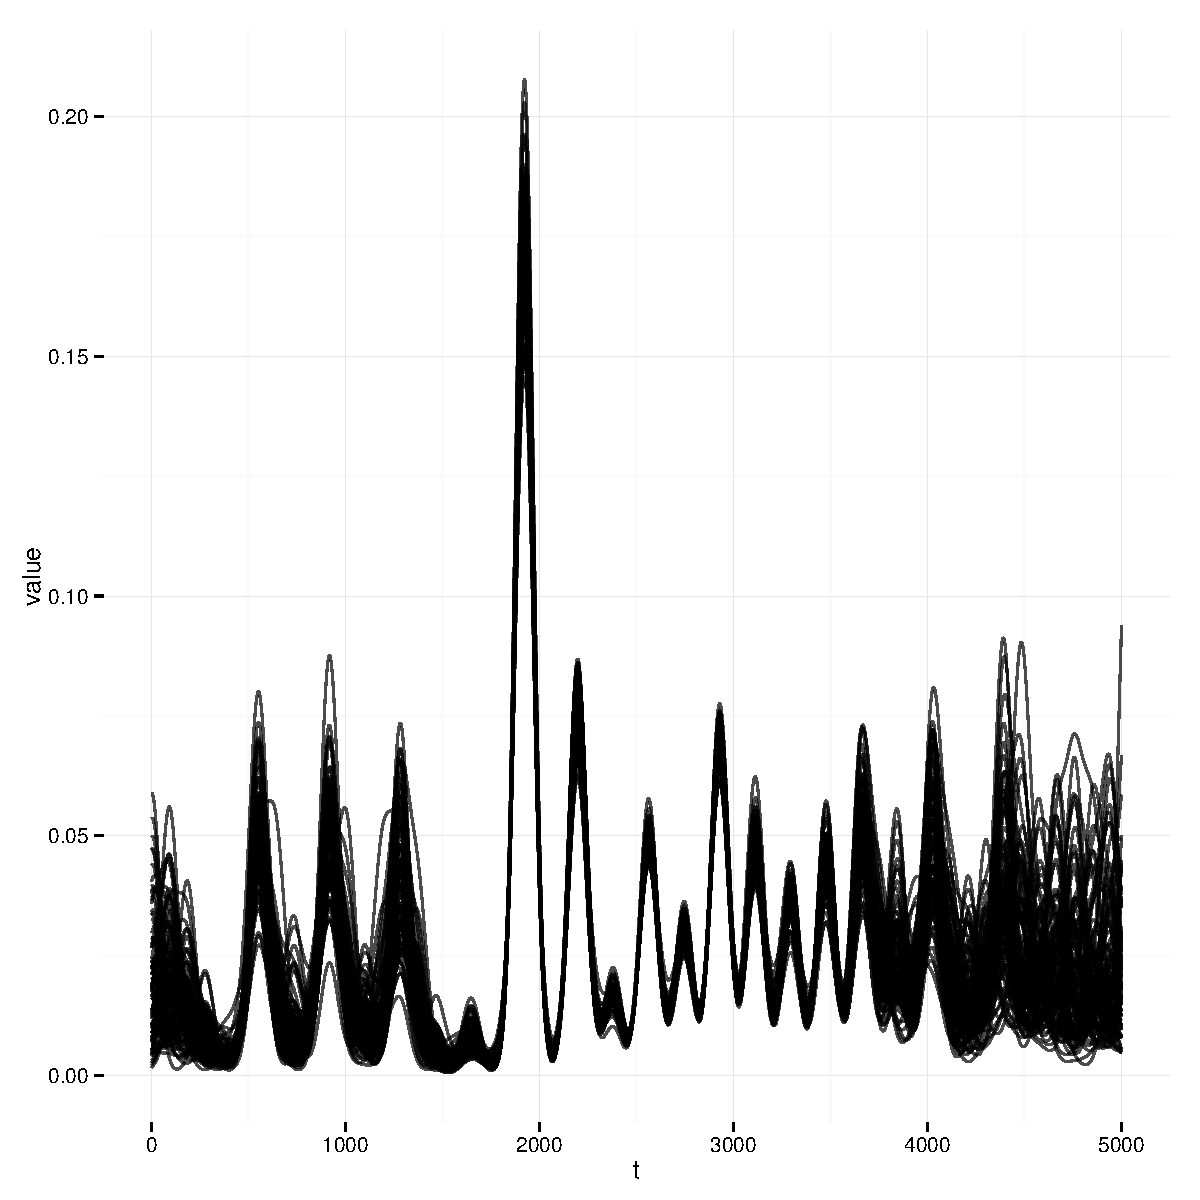
\includegraphics[clip, trim=0 0 0 200, width=\textwidth]{local-model.pdf}
  	\end{figure}
  
\end{frame}


\begin{frame}{survival response surface}
  \framesubtitle{modified cjs, local response model}

	\begin{figure}
	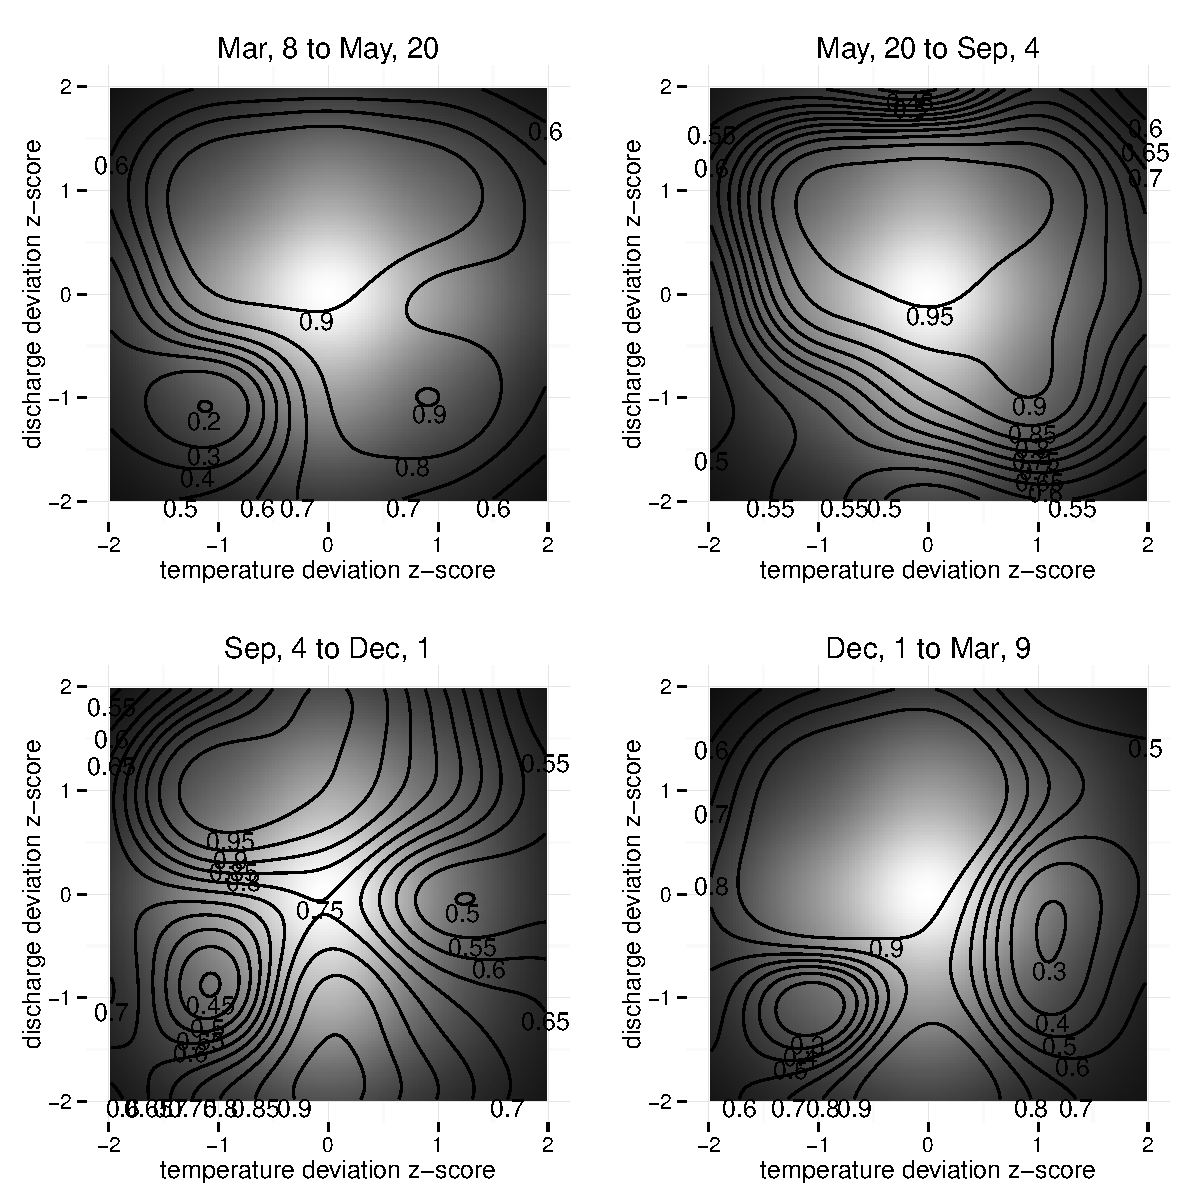
\includegraphics[clip, trim=0 0 0 35, height=.8\textheight]{donut-environmental-effect-on-survival.pdf}
  	\end{figure}

\end{frame}

\begin{frame}{survival response surface}
  \framesubtitle{modified cjs, local response model}

	\begin{figure}
	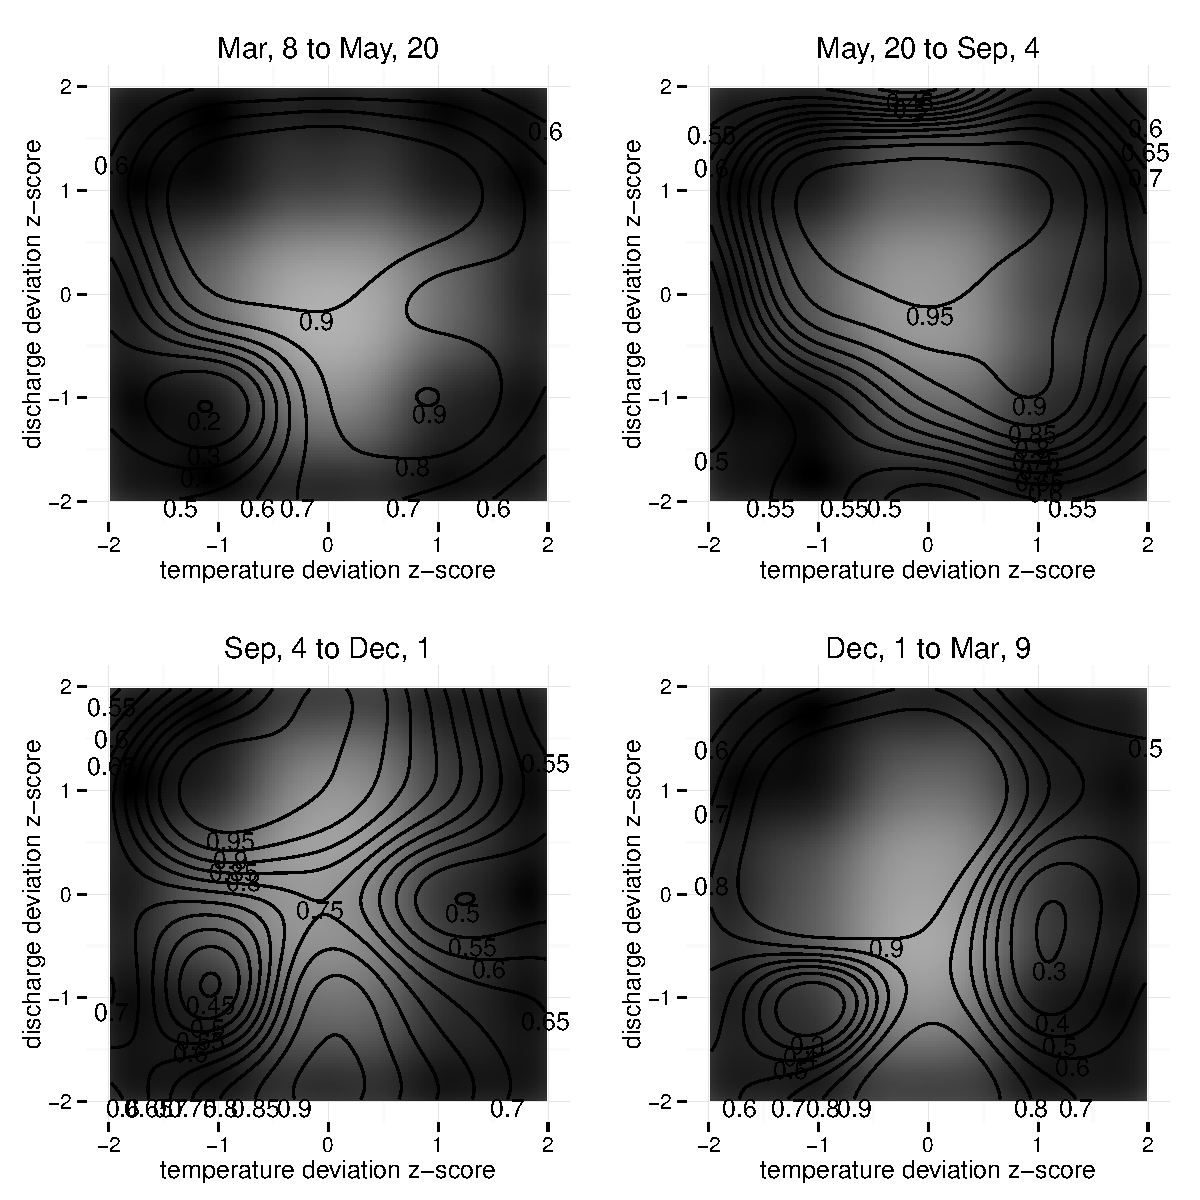
\includegraphics[clip, trim=0 0 0 35, height=.8\textheight]{donut-environmental-effect-on-survival-wu.pdf}
  	\end{figure}

\end{frame}



\begin{frame}{References}

    \begin{description}
    \item [imgc.allpostersimages.com] thanks for all the bears.
    \item [Houston, DeAgnerlis, Post (1988)] New Computer Models Unify Ecological Theory. BioScience. 38(10) 682--691]
    \item [Randin et al. (2006)] 
    \item [Sundblad et al. (2009)] 
    \end{description}


\end{frame}





\end{document}